%% entwurf.tex
%% $Id: entwurf.tex 28 2007-01-18 16:31:32Z bless $
%%
%% ==============================
\chapter{Design and Analysis}
\label{ch:Design}
This master thesis aims to compare different positions on the ear for body temperature measurement. 
To achieve this, a prototype was developed in this master thesis, which allows temperature measurements at different positions in and around the ear. 
Subsequently, studies were conducted to collect temperature data at different locations in and around the ear and analyze the collected data.
Initially, this section outlines the OpenEarable platform, which constitutes the cornerstone for both the prototype and comprehension. 
Subsequently, the sensors crucial for temperature measurement are elaborated upon.
After laying the groundwork for understanding the prototype, the development and approach to designing the prototype is described.
In addition, the detailed methodology and procedure of the study are described.
The study results are described in chapter \ref{ch:Evaluation}.

\section{Platform: OpenEarable}
\label{ch:Design:Prototype:OpenEarable}
% Das OpenEarable ist ein vom TECO Institut eintworfener Prototyp, mit welchem es möglich ist, ohrbasierte Messungen durchzuführen. 
In Chapter \ref{Background:SensingWithEarables:OpenEarable}, the OpenEarable platform is thoroughly described, emphasizing its interaction with other components. 
The OpenEarable was designed for rapid prototyping and exploration of novel Earable applications, and this thesis successfully utilized it as the foundation for the prototype. 
Figure \ref{fig:design:prototype_connection} illustrates the seamless collaboration between all components. 
Leveraging an Arduino Nano 33 BLE, the OpenEarable enables the deployment of Arduino-based software, and its connection to both the PCB and FlexPCB is facilitated via the 4-pin connector. 
The developed software gathers data from the temperature sensors and effectively utilizes the OpenEarable's resources. 
The study data is persistently stored on the SD card, and the study termination is triggered by a double-click on the push button.
In summary, the OpenEarable platform proved to be a versatile and effective foundation for the prototype, enabling seamless interaction between its components and facilitating data collection from the temperature sensors. 
By leveraging Arduino-based features and user-friendly design, OpenEarable was successfully used in this study to explore novel Earable applications and conduct the user study easily and efficiently.

% TODO: PCB Schematic in den Anhang vermutlich packen, sehr wichtig!!!

\section{Sensors}
\label{ch:Design:Prototype:Sensors}

Based on research and experience at the TECO Institute, the MLX90632 sensor was selected for its suitability for our project.

The MLX90632 sensor is an infrared temperature sensor known for its high accuracy in temperature measurements. This enables reliable applications where precise temperature tracking is needed.
Furthermore, non-contact temperature measurement is a huge advantage. 
The MLX90632 can measure temperature without physical contact with the object or body part, providing a non-invasive and convenient ear temperature monitoring option.
In order to place the temperature sensors in the necessary locations to measure temperature, the sensors must be appropriately small. 
Since the MLX90632 has a small form factor, this is optimal for the application needed.
Additionally, the MLX90632 is readily available on the market and has existing Arduino libraries. 
This availability and compatibility with Arduino simplify the integration process and save valuable development time.
In addition, the sensor is designed for low power consumption, making it suitable for battery-powered devices. 
Given the small battery size in the developed prototype, low power consumption is critical for extended operation during the study.
The MLX90632 offers fast response times and allows for real-time temperature monitoring and fast updates. 
Some difficulties arose when writing the EEPROM, so the default value was left at 2Hz.
The intention of adjusting the measuring rate was the implementation details of the library, which was finally solved by adjusting the library. 
This process is described in more detail in the chapter \ref{ch:Implementation}.
The high sensitivity to temperature changes allows the MLX90632 to accurately detect even minor variations. 
This sensitivity is advantageous for precise temperature tracking.
In addition, the sensor has applications in both the consumer and industrial markets due to its accuracy and reliability. 
This versatility makes it an excellent choice for our master's thesis project, which involves working with an Arduino Nano 33 BLE.

The MLX90632 has 4 pins that must be connected. Beside 3.3V and Ground the MLX90632 has a SCL and SDA connector. 
SCL stands for the clock signal, and SDA for the data flow.

Overall, infrared temperature sensing capabilities, accuracy, easy availability, non-invasive measurement, compact size, and compatibility with Arduino make the MLX90632 an ideal choice for the developing ear temperature monitoring system.

\subsection{Calibration Mechanism for Sensor Fusion}
\label{ch:Design:Prototype:Sensors:Calibration}
In the context of this study, the primary focus was on investigating the variability of temperature measurements at diverse positions in and around the ear, rather than obtaining a universally accurate temperature value. 
The sensors used had a factory accuracy of \( \pm0.2^\circ \text{C} \), but showed variability of up to \(1.1^\circ \text{C}\) under controlled conditions in preliminary self-tests. 
This motivated the implementation of a calibration mechanism to harmonize the sensor data. 
Different reference temperatures ($25, 30, 35, 40, 45^\circ$ C) and fitting models, varying from constant and linear offsets to polynomial offsets of different degrees (2, 4, 8, 16, 32), were used for calibration. 
The sensors were placed at uniform distances from a tempered metal plate to quantify systematic differences. 
Despite the controlled experimental setup, significant discrepancies were found between sensor readings, highlighting the need for an internal calibration mechanism to improve data consistency across multiple measurement locations.

Data logging was performed for calibration. 
The sensors, before being installed in the prototype, were arranged so that they were all positioned on a metal surface and aligned at an equal distance from another metal plate.
This was to take advantage of the thermal properties of the metal to obtain consistent temperature measurements across all 6 sensors.
The target metal plate was set to different reference temperatures ($25, 30, 35, 40, 45^\circ$ C) and a series of measurements was started.
Then, the recorded measurement data were concatenated and different offsets, including constant, linear and polynomial offset with the degrees (2, 4, 8, 16, 32), were calculated.

The MLX90632 sensor uses a special formula to convert measured values to temperature specifications, which is described in chapter \ref{ch:Design:Prototype:Sensors}.
Special attention is paid to the emissivity factor, a dimensionless quantity between 0 and 1, which describes the ratio of the energy radiated from the surface to the energy of an ideal black body.
For measurements of body temperature, this factor must be set to 0.98.
Although the calibration was performed on metal, which requires an emissivity factor of 1, the factor was left at 0.98 to adapt the calibration to the human body.
The heated platform of a 3D printer served as the heat source for the metal plate, as it could cover the required temperature ranges.
The factors for the respective offsets were then saved in a JSON file, which can be used during analysis to calibrate the recorded data.

\section{Prototype}
\label{ch:Design:Prototype}
To measure the temperature as planned in Section \ref{ch:Introduction:PlannedApproach}, a custom-built prototype was developed as part of this master thesis.
The prototype consists of two components: an earpiece that resembles an in-ear headphone and a component placed behind the ear that resembles a hearing aid. TECO's OpenEarable platform for ear-based observations is integrated into the behind-the-ear component. This component serves as the central interface and houses the Arduino on which all code is executed. Additionally, a circuit board with three temperature sensors is connected to measure the temperature behind the ear.
The second component is placed in the ear and is also controlled by the OpenEarable via the Arduino Nano33 BLE installed there. The OpenEarable acts as the basis for reading and storing data from the sensors connected via I2C. The relationship and interaction of the components are visually represented in Figure \ref{fig:design:prototype_connection}.
To ensure functionality and protection of the hardware, custom 3D-printed enclosures were created for both the behind-the-ear component and the in-the-ear component. 
Figure \ref{fig:design:prototype_on_head_visual} shows the final result, worn by a participant, and also visually demonstrates the positioning of the components.
As shown in \ref{fig:design:prototype_on_head_visual}, the custom cases add durability and a high-end appearance to the product, improving its overall usability and aesthetics.
The use of the 8-pin cable effectively connects the two components, additionally ensuring good comfort.

\begin{figure}[t]
    \centering
    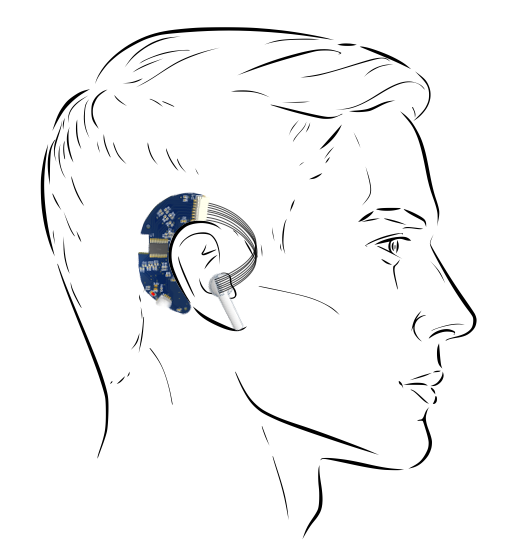
\includegraphics[width=0.48\textwidth]{thesis-doc/images/prototype/prototype_on_head_visual.png}
    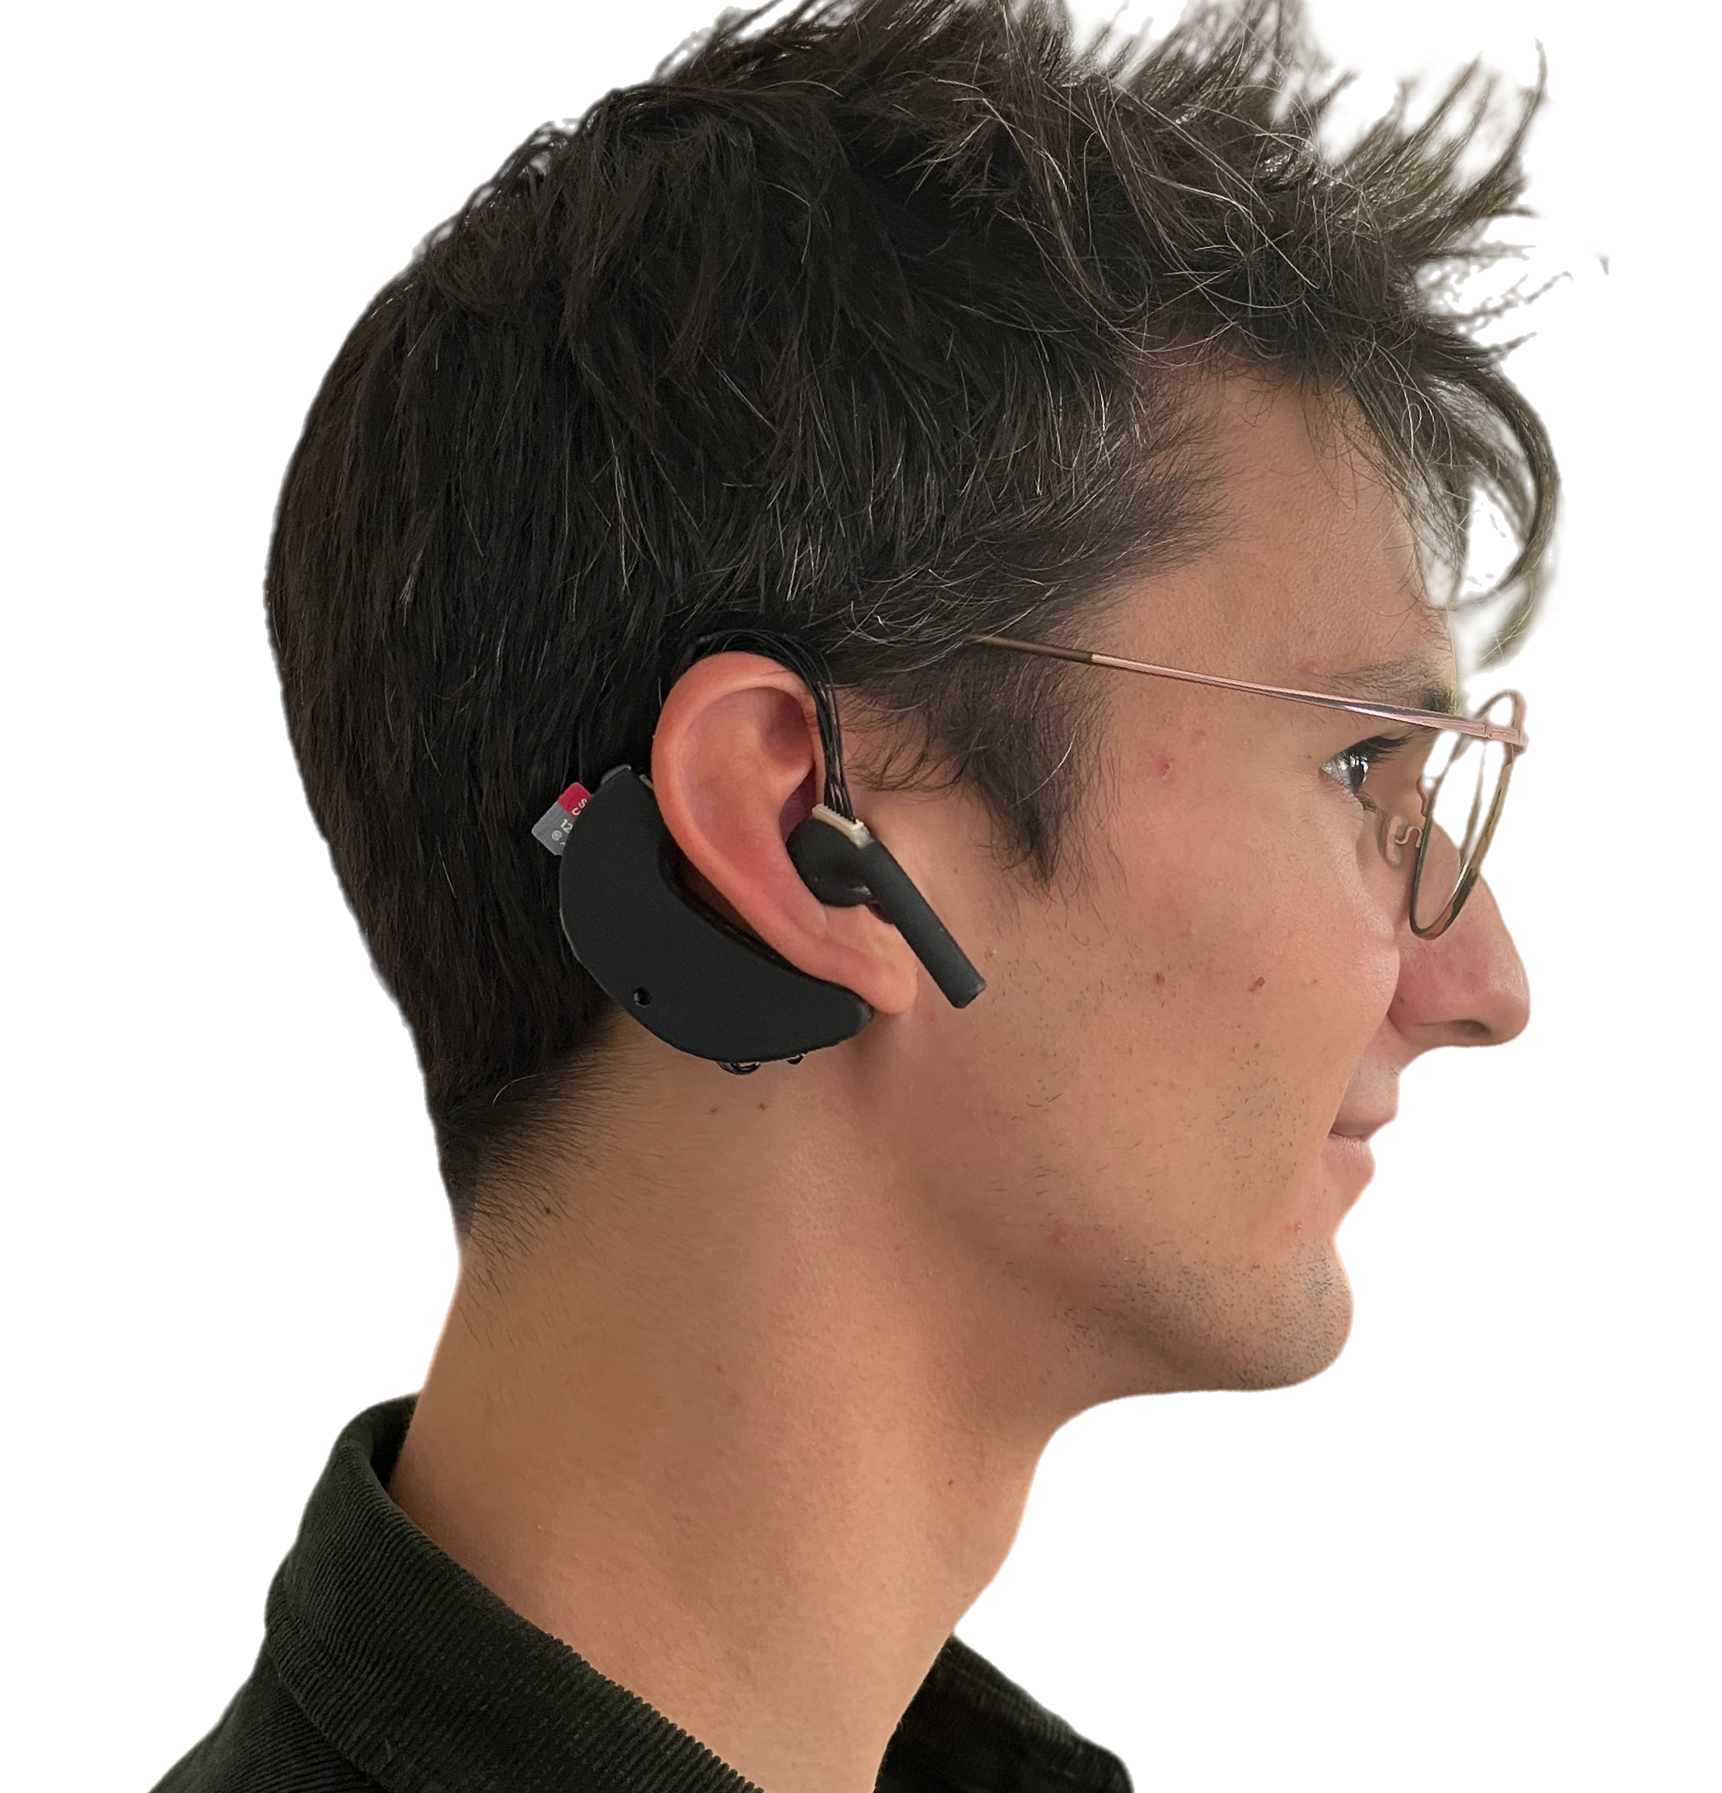
\includegraphics[width=0.48\textwidth]{thesis-doc/images/prototype/Lorenz.png}
    \caption{Visual view when theoretically carrying the components without wrapping the component behind the ear. The PCB behind the ear measures in 3 positions (bottom, middle, top) and is connected to the FlexPCB via an 8-pin connector, which is visually already wrapped in the sleeve here. The wiring of the two components results in good stability when worn, so the device cannot fall off. In addition to this visual representation, the prototype can be seen in a real environment including the cases.}
    \label{fig:design:prototype_on_head_visual}
\end{figure}

\begin{figure}
    \centering
    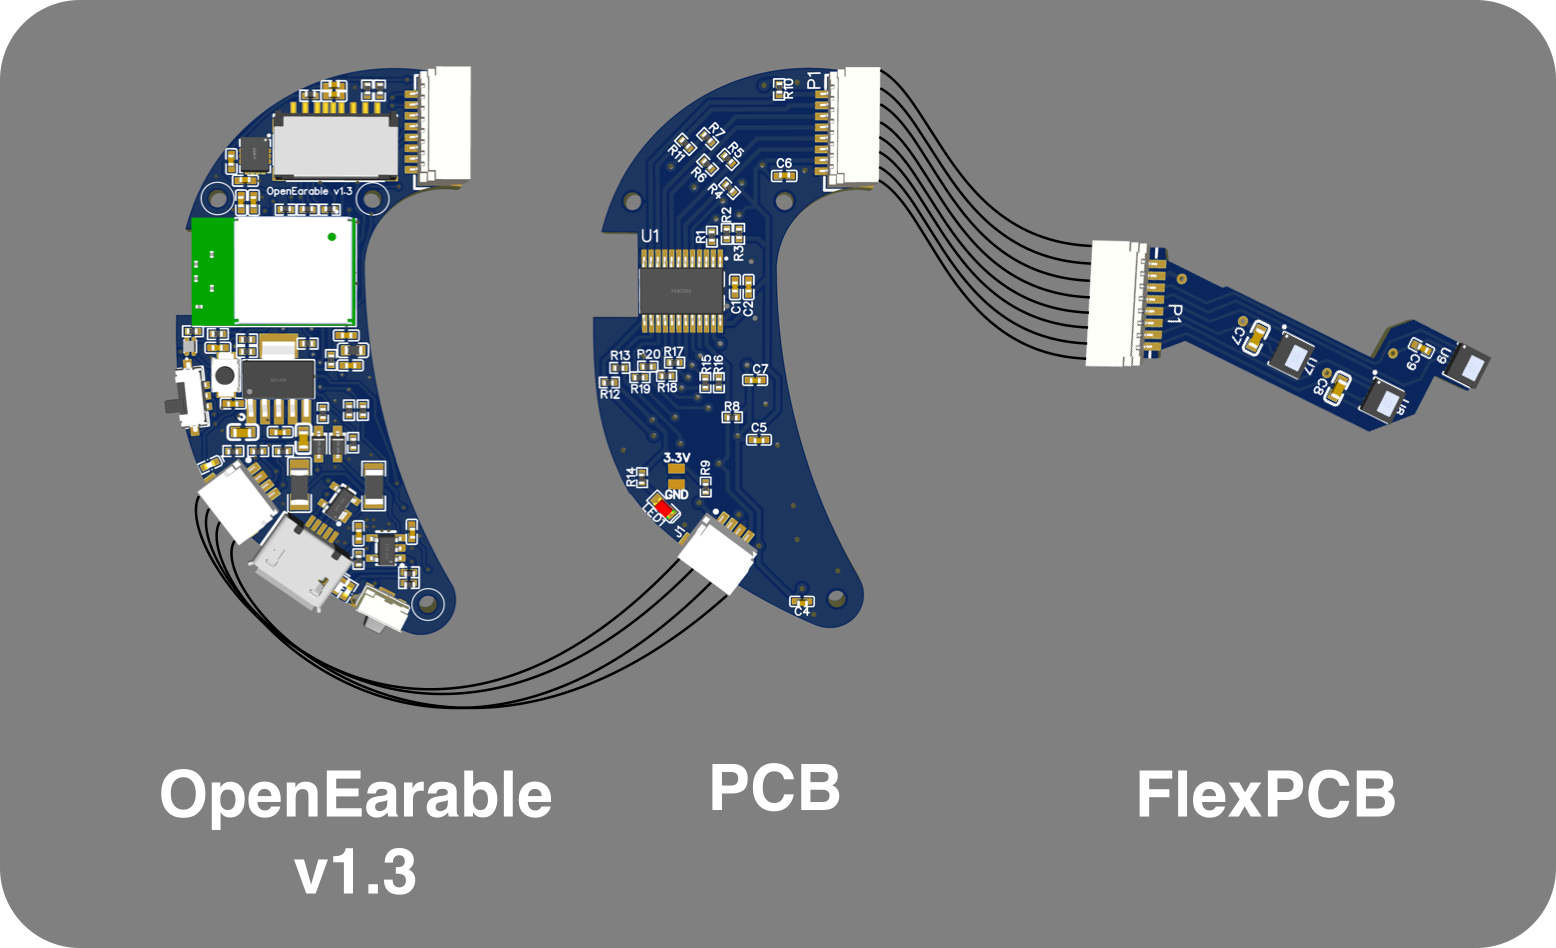
\includegraphics[width=\textwidth]{thesis-doc/images/prototype/PrototypeConnection.png}
    \caption{Visual representation of the prototype and the interaction of all components. The PCB is connected to the OpenEarable v1.3 with a 4-pin connector. In the OpenEarable is an Arduino Nano33 BLE, with which it is possible to control the multiplexer (TCA9548A) via I2C. Through this, every sensor value on the PCB and also on the FlexPCB can be read out, since the FlexPCB is also connected to the multiplexer via the 8-pin connector.}
    \label{fig:design:prototype_connection}
\end{figure}

\begin{figure}
    \centering
    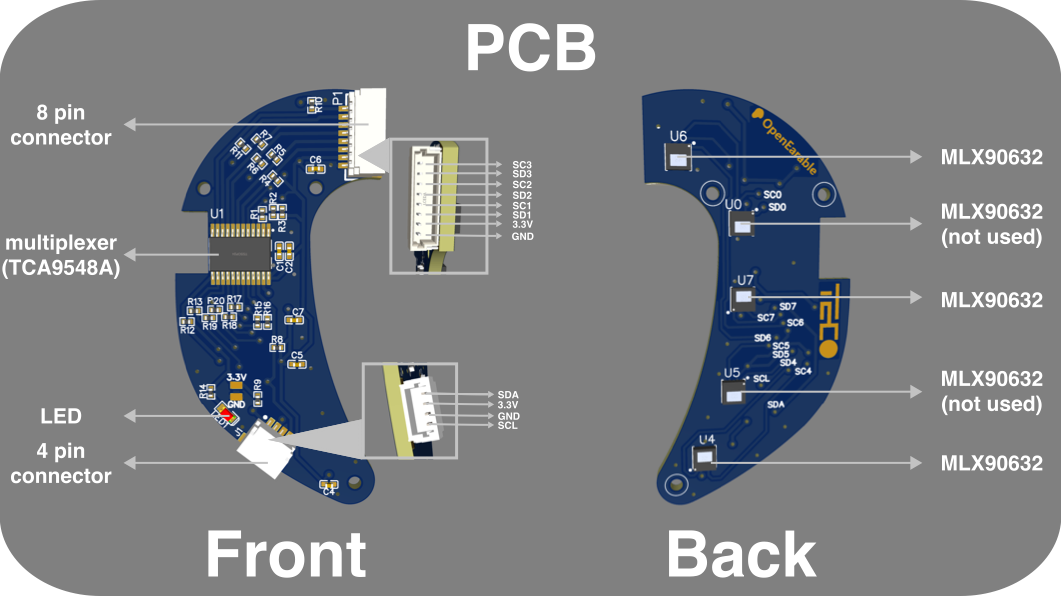
\includegraphics[width=\textwidth]{thesis-doc/images/prototype/PCB_Description.png}
    \caption{Representation of the front and back of the PCB. The multiplexer can be seen on the front, which is controlled by the OpenEarable via the 4-pin connector. The three other MLX90632 are then connected by the FlexPCB via the 8-pin connector. In addition, an LED is connected to the front, which lights up green if no short circuit is generated. The temperature sensors can be seen on the back, but only three of the five connections visible in the design are used.}
    \label{fig:design:pcb_description}
\end{figure}

\subsection{Temperature Measurements Behind the Ear}
\label{ch:Design:Prototype:BehindEar}

The temperature behind the ear is measured at 3 positions, as can be seen in Figure \ref{fig:design:pcb_description} on the back of the PCB.
To position the temperature sensors at the locations chosen in section \ref{ch:Introduction:PlannedApproach}, a PCB was developed that has the sensors installed at the appropriate locations. 
The PCB has been designed so that only the temperature sensors are placed on the back. This allows the PCB to be placed entirely in the bottom of the case, while the temperature sensors peek out through matching openings in the case. On the front of the PCB are all the other components, including a 4-pin connector and an 8-pin connector.
The 4-pin connector is used to connect to the OpenEarable. This connection allows the OpenEarable to communicate with the PCB via I2C, as the OpenEarable also has a special 4-pin connector for this purpose.
To be able to control the second component (the earpiece) via I2C later on as well, the 8-pin connector was added to establish a connection to the second component.
Via I2C, the built-in multiplexer is addressed, with which one of the eight possible applied lines can be switched and read out. The eight possible through-connections of the multiplexer are connected to all temperature sensors, including those of the FlexPCB via the 8-pin connector.
In addition, an LED is installed on the PCB to directly indicate a possible short circuit.
For each temperature sensor, the signals Ground, Power (3.3V) as well as SCL (clock signal) and SDA (data transmission) are required, as shown in Figure \ref{fig:design:pcb_description}. Communication with the multiplexer can be handled through the 4-pin connector.
To connect the 3 temperature sensors of the FlexPCB, a total of 12 signals are required, which can be reduced somewhat. For this purpose, the ground and power signals can be used together, resulting in a total of 8 signals being transmitted.

A case has now been developed around the OpenEarable and the custom-made PCB to enable a comfortable fit.
Above the PCB, the battery is placed in the enclosure so that no long cables are needed for the power supply to record the data in the study conducted.
The OpenEarable is placed above this.
The dimensions of the PCB are exactly the same as the OpenEarable to keep the case as small and compact as possible.
The sensor used requires an angle of $ 50 ^ \circ$ around itself for the temperature to be reliably measured. 
This was taken into account.
The layered representation for visualization can be seen in Figure \ref{fig:design:prototype_behind_head_layered_view}.

\begin{figure}
    \centering
    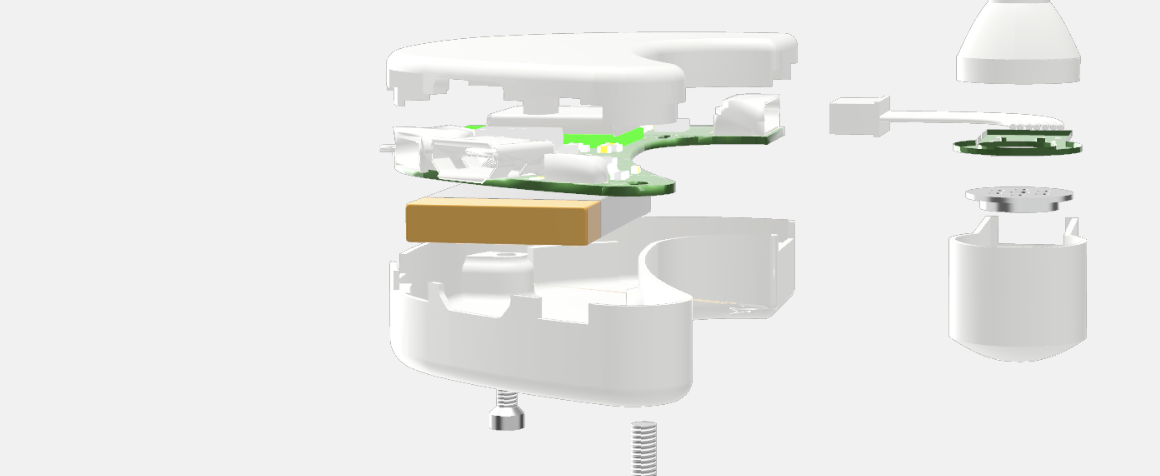
\includegraphics[width=\textwidth]{thesis-doc/images/prototype/Prototype_PCB_layered_view.png}
    \caption{Layered view of the component behind the ear. At the bottom is the designed PCB as the temperature sensors can look out towards the skin. The battery is placed between the PCB and the OpenEarable.}
    \label{fig:design:prototype_behind_head_layered_view}
\end{figure}

\subsection{Temperature Measurements in the Ear}
\label{ch:Design:Prototype:Earpiece}

The second component now enables temperature measurement in the ear area. The FlexPCB itself is only equipped with components on the front side. Thereby, the 8-pin connector that connects the FlexPCB to the PCB is located, as described in section \ref{ch:Design:Prototype:BehindEar}. Additionally, three temperature sensors are placed on the FlexPCB to sense the positions in the ear and pinna described in section \ref{ch:Introduction:PlannedApproach} and Figure \ref{fig:ear_measurement_positions}.
The FlexPCB was designed to extend through the component. On the one hand, the 8-pin connector protrudes outward to connect to the PCB. On the other hand, the PCB runs along the outside of the housing to the earbud, allowing the FlexPCB to snake through. The tip of the FlexPCB also contains a temperature sensor mounted in the earplug and aimed directly at the eardrum. Another temperature sensor is aimed at the ear canal and is located on the outer edge of the earplug. The third temperature sensor is aimed at the pinna.
The component was modeled on the design of an AirPod, but heavily modified afterward. The original AirPods design is freely available on TinkerCAD and was used as the basis for the component shape. The inside of the design was completely hollowed out to allow cables to be routed through the case. Additionally, an adapter was added to the side to fit the redesigned earpod. An earbud can be attached here to ensure that the earbud penetrates further into the ear than usual compared to conventional in-ear headphones. This enables precise temperature measurement in the direction of the eardrum. A temperature sensor is attached to the tip of the earbud to perform basic temperature measurements.
The three temperature sensors on the FlexPCB can be switched via the multiplexer that is connected to the PCB. This allows for precise selection and acquisition of the desired measurements. Figure \ref{fig:design:prototype_earpiece_views} shows a sketch and other images of the final component.

\begin{figure}[!h]
    \centering
    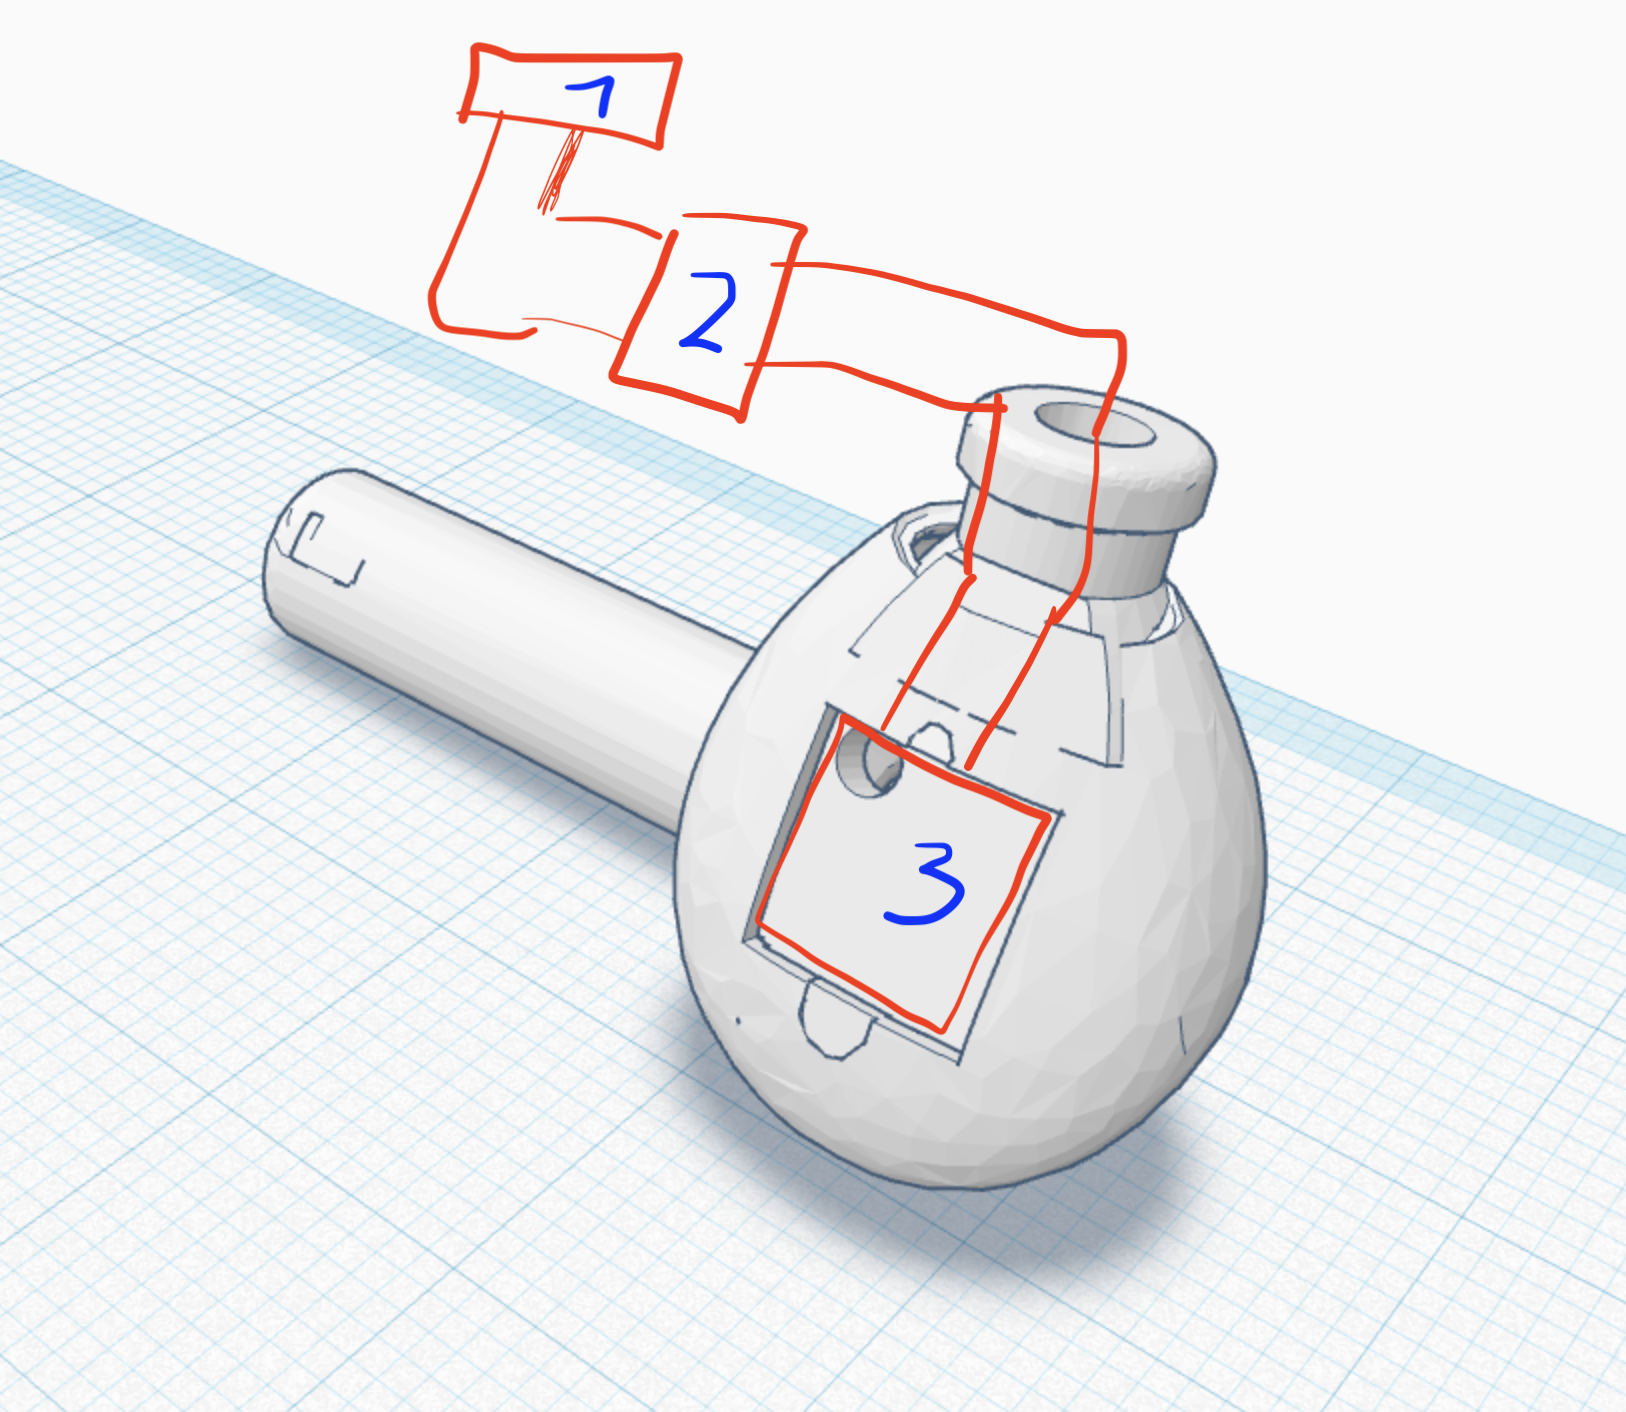
\includegraphics[width=0.48\textwidth]{thesis-doc/images/prototype/flex_pcb_design_finding.png}
    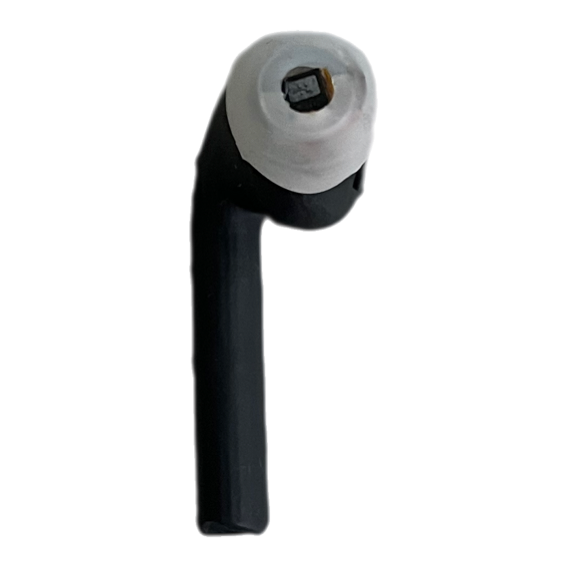
\includegraphics[width=0.48\textwidth]{thesis-doc/images/prototype/Earpod_Front.png}
    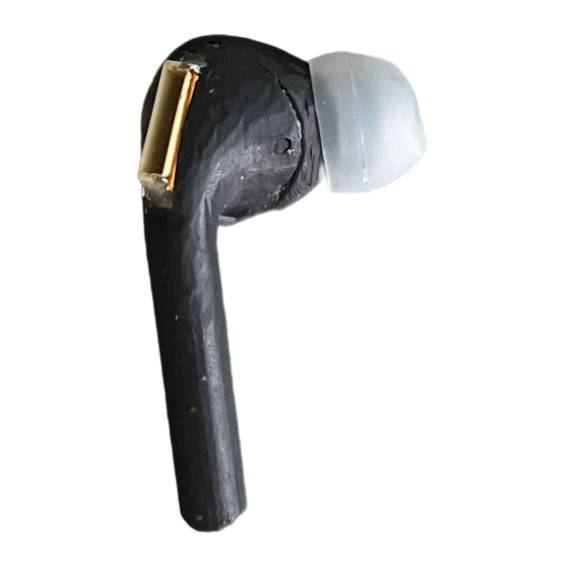
\includegraphics[width=0.48\textwidth]{thesis-doc/images/prototype/Earpod_Side1.png}
    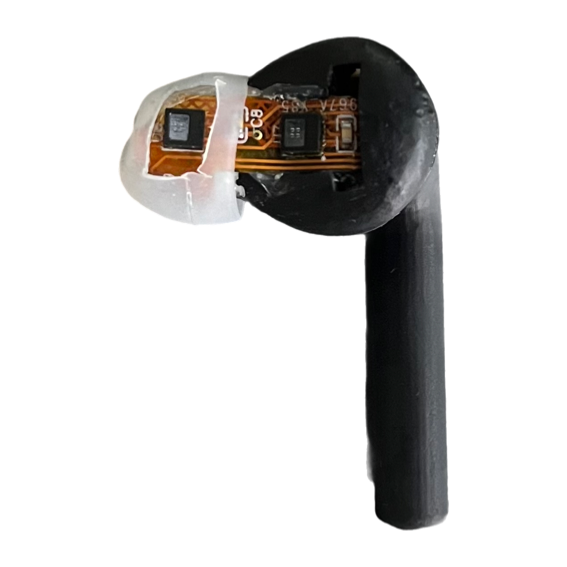
\includegraphics[width=0.48\textwidth]{thesis-doc/images/prototype/Earpod_Side2.png}
    \caption{Sketch and real view of the earpiece from different perspectives.
The sketch shows the first idea of how the FlexPCB has to be designed so that it gets through the earplug to the tip to measure in the direction of the tympanic membrane. The real views provide an impression of how the component is composed. On the bottom right picture, you can see the sensors on the concha and ear canal, on the top right picture the sensor directing to the tympanic membrane. The bottom left picture displays the 8-pin connector.}
    \label{fig:design:prototype_earpiece_views}
\end{figure}

\section{Study}
\label{ch:Design:Study}
The requirement of this master thesis is to measure the temperature at different positions of the ear to enable temperature measurement over a longer period of time. 
For this purpose, a study is to be conducted in which the temperature is measured at different positions and then compared. 
For this purpose, a prototype was developed, which was described in detail in the previous chapters. 
With this prototype, it is possible to measure the temperature at three positions behind the ear, on the auricle, in the ear canal and on the eardrum.
The goal after recording the data is to compare the different positions. 
In the context of this master's thesis and related study, several hypotheses arise that have the potential to clarify key aspects of ear temperature measurement. 
One of these hypotheses concerns location-dependent temperature accuracy. It is hypothesized that the position of the sensors, whether behind the ear, in the pinna, in the ear canal, or on the eardrum, significantly affects the accuracy of the temperature measurement.
Furthermore, the question of replicability and consistency of the measurements is of interest. It is assumed that despite the variable human physiology, the measurement results are consistent across different subjects. The relevance of the initial acclimatization phase of the sensors is also considered. Here, it is assumed that the 20-minute acclimatization phase is sufficient to ensure stable temperature measurement. 
The role of environmental variables is also considered. 
It is hypothesized that the readings could differ significantly from the baseline measurements after being outdoors, allowing conclusions to be drawn about the susceptibility of the sensors to environmental conditions. 
In addition, the adaptability of the measurements to changing temperature conditions is another key issue. 
It is hypothesized that the sensors will respond quickly enough to detect and account for changes in ambient temperature while outdoors.
In the context of the further hypotheses, for example, the question is raised whether changes in the IMU signal, i.e. in the gyroscope, magnetometer and accelerometer measurements, are correlated with changes in temperature. Similarly, the relevance of the physiological nature of the subjects, such as the skin thickness behind the ear or the ear shape, is highlighted in relation to the measurement accuracy. 
Finally, the speed of the sensors in detecting rapid temperature changes induced by physical or emotional states is considered as a possible variable for assessing system performance.
These hypotheses not only provide a broad basis for evaluating the developed prototype, but can also be used to define further research questions and applications in the field of temperature measurement by wearables.

\subsection{Study 1: Localized Ear Temperature Measurement Study Procedure: Baseline Surveys and Environmental Influences}
\label{ch:Design:Study:Study1}

Two studies were conducted as part of this master's thesis. 
The first study deals with the comparison of the temperatures at the different positions.

For this purpose, a study was designed to test the different hyptotheses and to create the best possible data basis. 
The study starts with the temperature measurement of the right ear by a thermometer (BRAUN ThermoScan 7) to obtain a reference value of the temperature in the ear. 
This measurement will be taken again at the conclusion of the study.
This is followed by the attachment of the prototype to the subject's ear. This phase is critical, as correct positioning of the sensors is crucial for the quality of the recorded data.
Since the component behind the ear tends to stick out a bit from the skin after a while, the component was taped behind the ear to be securely in the correct position and not slip even during light activities. 
After the installation of the prototype, an acclimatization phase of 20 minutes follows, during which data is already recorded \ref{chagllae.MeasurementCoreBody2018}. 
This phase is to ensure that the sensors have sufficient time to adapt to the physiological conditions of the subject and to allow stable measurements.
After completion of the acclimatization phase, the main data collection is performed. 
The subject spends another 20 minutes in a seated position in a room of the institute where all other subjects have also performed the study. 
The room is not air-conditioned and the windows were closed before the measurement.
In addition, the room temperature and humidity were noted. 
This phase is to provide a baseline for the temperature measurements and to verify the consistency of the sensors under stable conditions.
The next step is to investigate the influence of environmental variables. 
Subjects will be asked to spend time outdoors walking for 20 minutes. 
This is done to analyze the response of the sensors to sudden changes in temperature and environment and to evaluate the adaptability of the system.
After returning indoors, subjects again sit in their original seats and remain in a seated position for another 20 minutes. 
This phase allowed for quantification and analysis of any deviations in sensor measurements due to being outdoors.
Throughout the time in the room, subjects were allowed to watch animal documentaries that allowed for no or minimal anxiety or happiness. 
In total, the study will be conducted with 15 subjects to provide a sufficient database for statistical analyses.

Through this carefully designed procedure, the study is expected to help test the formulated hypotheses and provide valuable insight into the performance of the developed prototype and its potential applications.

\subsection{Study 2: Study Course Under Stress Conditions: Impact on Temperature Measurements With Ear-Based Sensors}
\label{ch:Design:Study:Study2}
In the second study, the influence of stress-induced physiological changes on temperature measurements at different sites of the ear is investigated. 
An initial 20-minute acclimatization period, during which the sensors and the subjects adapt to the environmental conditions, is followed by a 15-minute measurement period in a seated position.
After that, the subjects are exposed to a stress situation. 
At the beginning of the stress phase, the subjects solve a Stroop test, then an N-Back test and finally a mathematics test. 
The Stroop test tests the subjects' attention by alternately displaying words in different colors. 
The subject is asked to interpret the color of the word. The words are always color words, but the words do not always match the color in which they are displayed. 
When the word and the color do not match, the reaction time and the number of errors increase. 
This is to create an initial stress situation for the subject \cite{StroopCompetitionSocialEvaluative}. 
Next, an N-back test with 2 dimensions is performed. 
Here, a letter is named to the subject via a voice output and a position in a tic-tac-toe field is displayed. 
The subject must now recall N steps back and indicate whether the letter or position has already been named or shown in the last N iterations. 
This test was performed with $N={1,2,3}$ and is designed to elicit strain and stress \cite{liangEffectAcuteStress2023}.
Last, the subject is presented with a mathematical test. 
This involves several mathematical tasks in which 4 answer options are always available.
Here, the subject has 8 minutes to solve as many tasks as possible. 
This is also designed to trigger a stress situation \cite{caviolaStressTimePressure2017}.
The three tests are all designed to trigger stressful situations and always challenge the subject in a different way.
For the Stroop test, there is no visual timer, but the number of words is limited. 
There is a high score for the test, which is intended to motivate the subject to do as well as possible. 
In the N-Back test, the time is strictly given, the subject has the opportunity to answer within 3 seconds.
Here, the subject is exposed to the risk of being frustrated if he or she fails to complete one or more sub-steps.
The mathematical test has a time limit of 8 minutes, in which the subject must solve as many tasks as possible.
Again, the subject is put under pressure in a different way that is intended to trigger stressful situations.
This scenario was chosen because a large study was not possible due to time constraints. 
Standard in science for induction in standardized stress induction tests is the Trier Social Stress Test (TSST). 
However, the selected test covers the requirements and should allow to induce stress in the subjects.
To check the stress level of the subjects, heart rate is measured in addition to temperature data. 
These additional markers provide a solid scientific basis for evaluating stress induction and its effects on the measured temperature values.
The stress induction phase is followed by another 15-minute measurement phase in a seated position, during which the subjects are not exposed to any other stressful situations. 
This serves to record the recovery processes and their effects on the measured parameters. 
In study 2, the effect of different stress-inducing tests - the Stroop test, the N-back test and a timed mathematical test - on the temperature measurement at the ear is investigated.
At the same time, heart rate will be measured as an additional physiological marker of stress. 
The study includes an initial acclimation phase, a pre-stress measurement phase, a stress induction phase, and a post-stress measurement phase to comprehensively assess ear temperature variations under stress conditions.